\documentclass[prd, nofootinbib, floatfix, 11pt, tightenlines, times]{article}
\usepackage[paperwidth=8.5in,paperheight=11in,centering,margin=1.0in]{geometry}
\usepackage[pdftex]{graphicx}
\usepackage{natbib}
\usepackage[toc,page]{appendix}
\usepackage{subfig}

% pdflatex W14report.tex; bibtex W14report; pdflatex W14report; pdflatex W14report

% Border around the figures
%\usepackage{float}
%\floatstyle{boxed}
%\restylefloat{figure}

\def\figdir{../figures}
\def\pasp{{\it PASP}}
\def\A{{\tt A}}
\def\B{{\tt B}}
\def\C{{\tt C}}
\def\D{{\tt D}}
\def\E{{\tt E}}
\def\P{{\tt P}}

\title{\vspace{-22mm} \Large{Report on Winter2014 Production: Image Differencing} \vspace{-6mm}}
\date{\today}

\begin{document}
\maketitle
Summary

\clearpage
\tableofcontents
\clearpage

\section{Production Scope and Goals}
\subsection{Subtask 1: Reproduce W13 Results Using Current PhoSim}
\subsection{Subtask 2: Simulate Starfield using Multiple SEDs at a Single Airmass}
\subsection{Subtask 3: Simulate Starfield using Multiple SEDs at Multiple Airmasses}
\subsection{Subtask 4: Include Realistic Mix of Stars and Galaxies}
Pushed back to S14.
\section{Review of Wavelength Dependent Refraction}
\section{Running PhoSim}
\section{Analysis of Subtask 1}
\section{Analysis of Subtask 2}
\section{Analysis of Subtask 3}

\clearpage
\begin{figure}[h!]
  \centering
  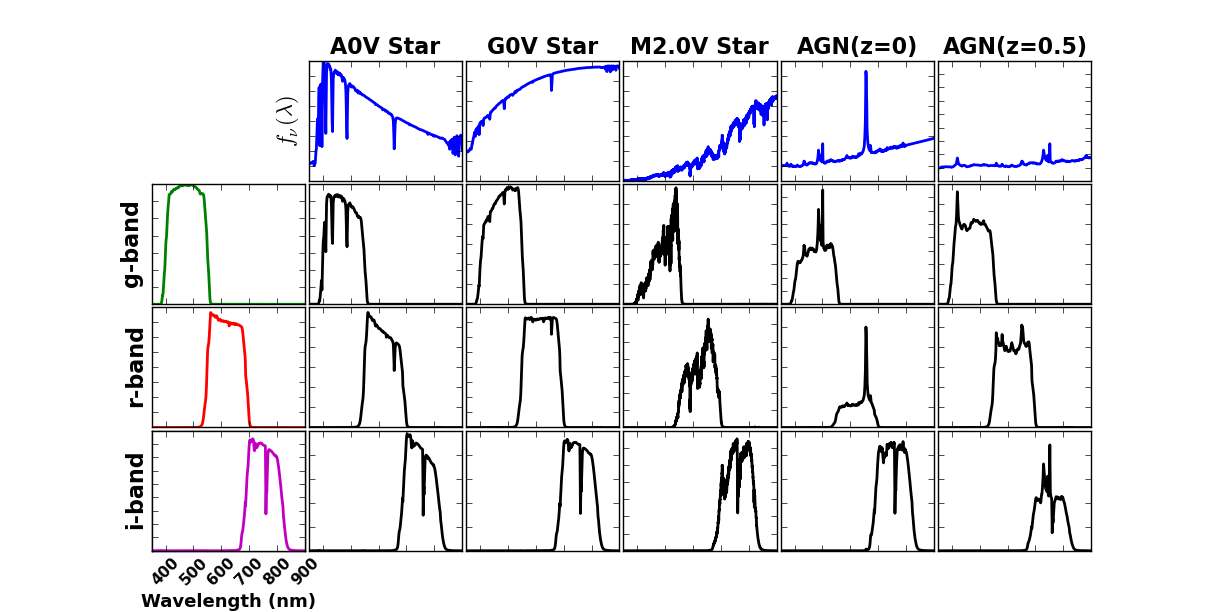
\includegraphics[width=1.1\textwidth]{\figdir/DCR1.png}
  \caption{{\bf Effective Spectral Energy Distributions} : The
    effective spectra of 5 reference objects -- a ``blue'' {\tt A0V},
    a reference {\tt G0V}, and a ``red'' {\tt M2.0V} star, along with
    a QSO at redshift $z=0$ and $z=0.5$ -- filtered through 3
    transmission profiles corresponding to the LSST $g$, $r$, and
    $i$--bands.  The top row shows the input spectral energy
    distribution $f_\nu(\lambda)$, while the leftmost column shows the
    LSST filter transmission profile in units of the normalized
    system response $\phi$.  The inner row,column figures show the
    effective spectrum of each SED (along columns) when multiplied
    through the respective filter (along rows).  In all subpanels, the
    x--axis is wavelength.  The {\tt A0V}, {\tt G0V}, and {\tt M2.0V}
    spectra correspond to {CAT\_SHARE\_DATA} files {\tt
      kp01\_9750.fits\_g45\_9830.gz}, {\tt
      km20\_6000.fits\_g30\_6020.gz}, and {\tt m2.0Full.dat.gz}
    respectively, and were used as the SEDs of the stars in the W14
    image simulations.  This figure may be recreated using the script
    {\tt python/DCR.py}.}
  \label{fig:spectra}
\end{figure}

\clearpage
\begin{figure}[h!]
  \centering
  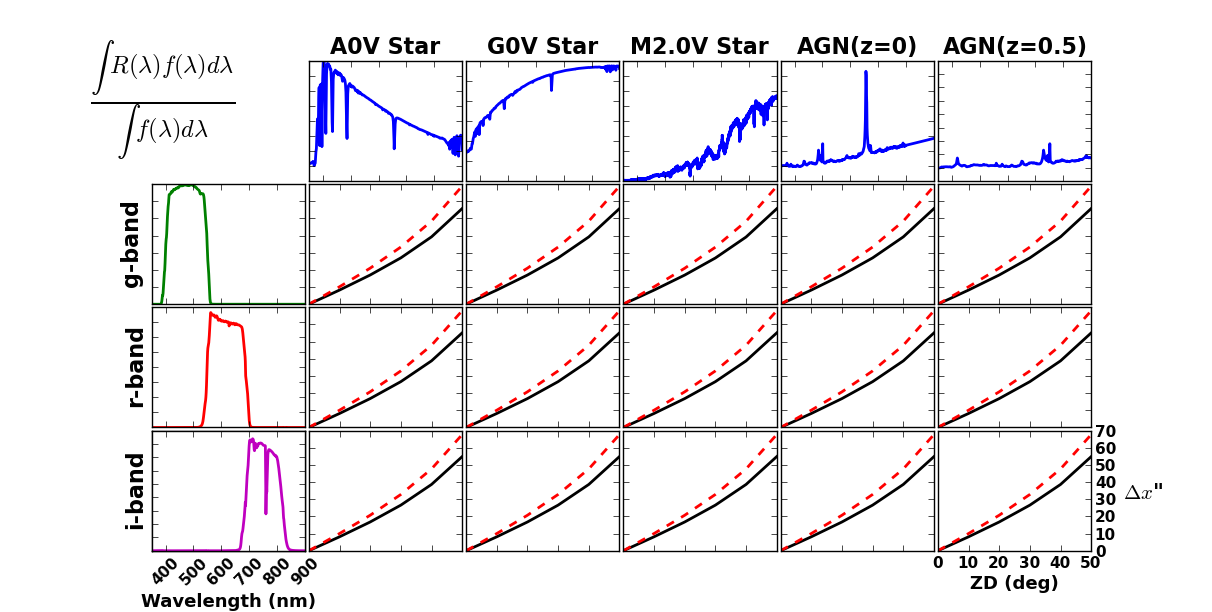
\includegraphics[width=1.1\textwidth]{\figdir/DCR2.png}
  \caption{{\bf Refraction Amplitude vs. Filter and Spectral Energy
      Distribution}: The flux-weighted amplitude of refraction (in
    arcseconds) for each of the filtered SEDs in
    Figure~\ref{fig:spectra}, as a function of zenith distance in
    degrees along the x--axis.  The solid black line is the nominal
    result from Eqn~\ref{eqn:dcr}, while the dashed red line ignores
    the corrections for temperature and pressure.  Note the maximum
    amplitude of refraction reaches nearly 1 arcminute.  This figure
    may be recreated using the script {\tt python/DCR.py}.}
  \label{fig:refraction}
\end{figure}

\clearpage
\begin{figure}[h!]
  \centering
  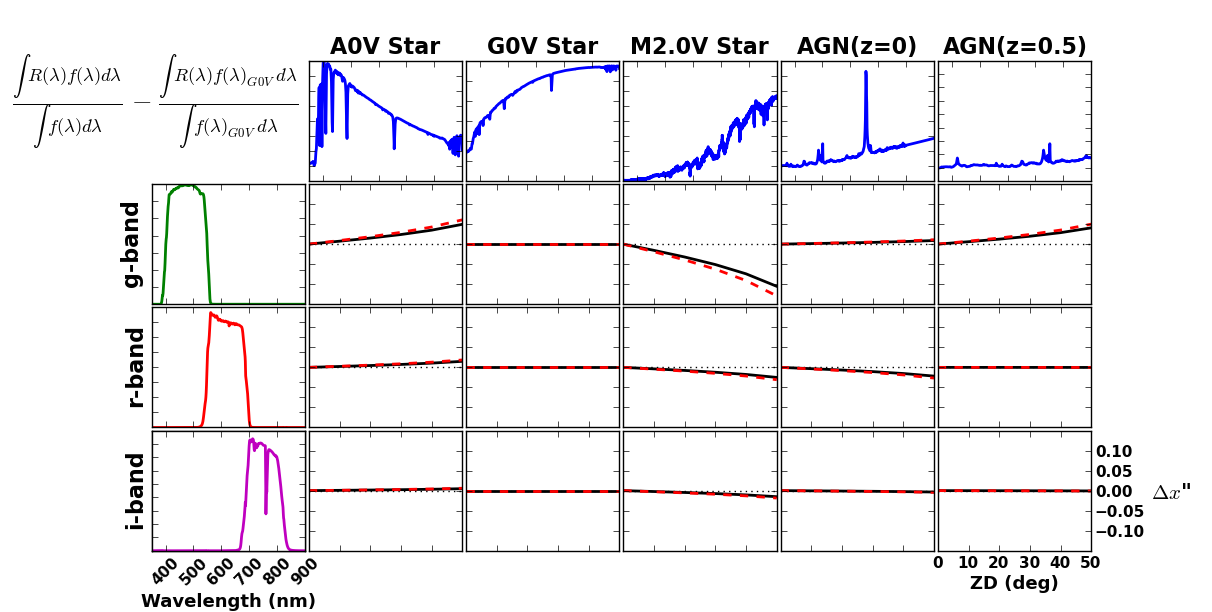
\includegraphics[width=1.1\textwidth]{\figdir/DCR3.png}
  \caption{{\bf Differential Chromatic Refraction vs. Filter and
      Spectral Energy Distribution}: The differential chromatic
    refraction of all sources from Figure~\ref{fig:spectra} with
    respect to the reference {\tt G0V} star, with respect to zenith
    distance.  The maximum amplitude of DCR reaches $0.1''$, or
    approximately half an LSST pixel.  This figure may be recreated
    using the script {\tt python/DCR.py}.}
  \label{fig:dcr}
\end{figure}

\begin{figure}[h!]
  \centering
  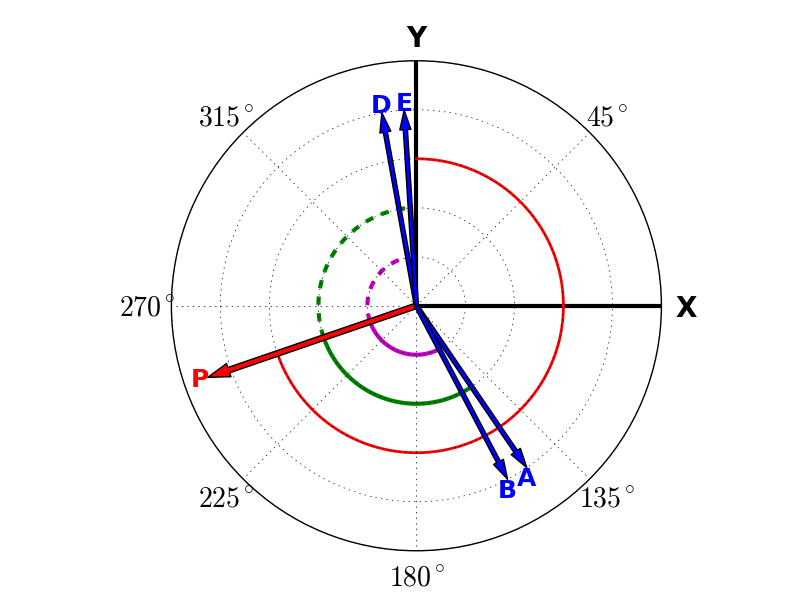
\includegraphics[width=1.1\textwidth]{\figdir/dcrPhoSim.png}
  \caption{{\bf Designed Orientation of Dcr in W14 Phosim Runs}: This
    figure represents the anticipated orientations of Dcr in the W14
    phoSim data.  The x,y coordinate system is depicted, as well as
    the convention that angles ({\tt rotTelPos}, {\tt rotSkyPos}) are
    clockwise with respect to the positive y--axis in the image
    coordinate system (counterclockwise in the camera coordinate
    system).  The {\tt rotTelPos} of 251 degrees specified for all
    simulations, which reflects the direction to the pole, is shown
    with the red vector \P and the red arc at y=0.6.  The derived {\tt
      rotSkyPos} for visits \A,\B,\D,\E\ are shown with the blue
    vectors, and reflect the angle towards zenith (the angle of
    increasing altitude).  Dcr is expected to happen along these
    vectors.  The angles \P\A,\P\E\ are similar, and represented by
    the green arcs; the angles \P\B,\P\D\ are also similar, and
    represented by the purple arcs.  This is expected as observations
    \A\ and \E\ are taken at airmass 1.55 (zenith distance of 50
    degrees) but at opposite sides of the meridian crossing of the
    star field; a similar situation was designed for observations
    \B\ and \D, which are taken at airmass 1.15 (zenith distance of 30
    degrees).  Visit \C\ is not depicted as it was taken at zenith.
    This figure was created using the script {\tt
      python/dcrSchematic.py}.}
  \label{fig:phosimdcr}
\end{figure}


\begin{figure}
    \centering
    \subfloat[Visit A]{{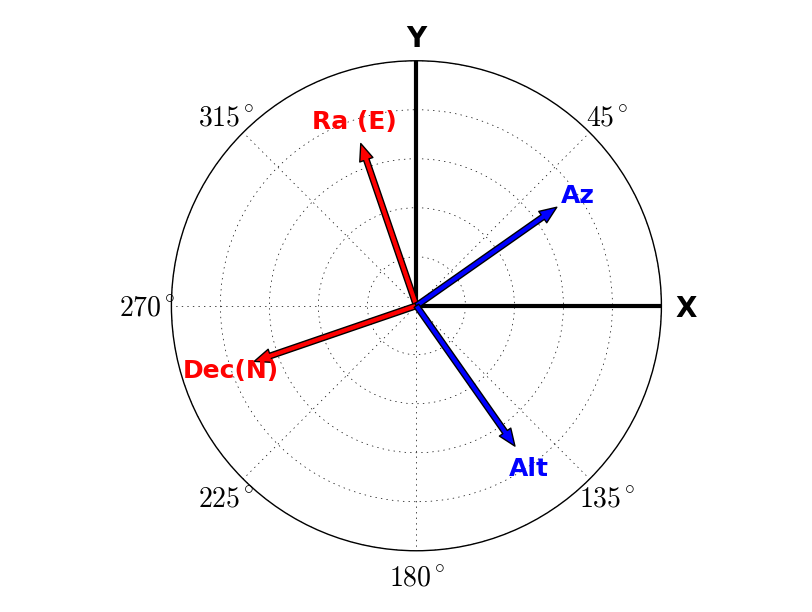
\includegraphics[width=0.46\textwidth]{\figdir/outputs8bCA_dcr_wcs.png} }}
    \qquad
    \subfloat[Visit B]{{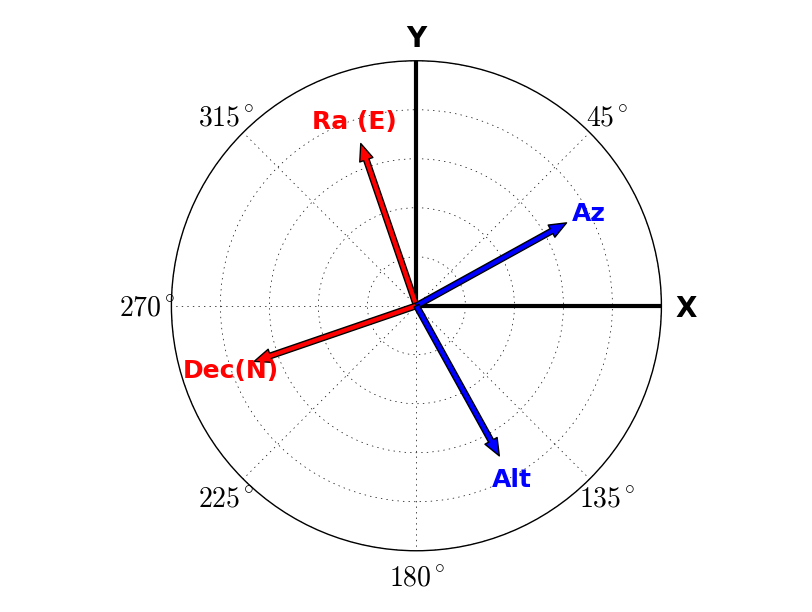
\includegraphics[width=0.46\textwidth]{\figdir/outputs8bCB_dcr_wcs.png} }} \\
    \subfloat[Visit D]{{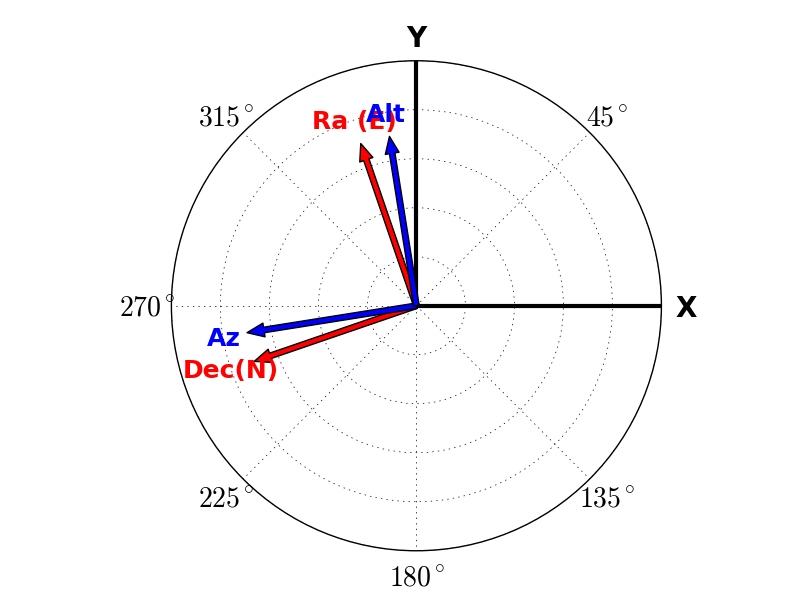
\includegraphics[width=0.46\textwidth]{\figdir/outputs8bCD_dcr_wcs.png} }}
    \qquad
    \subfloat[Visit E]{{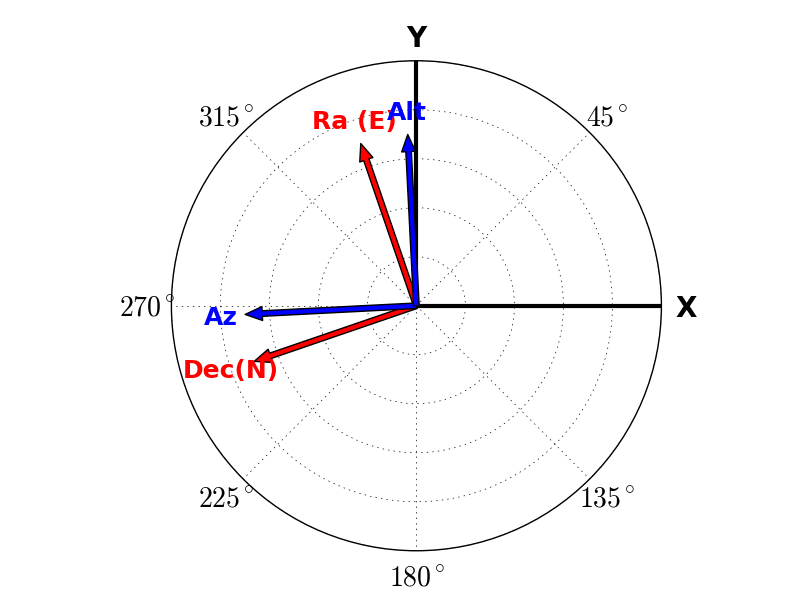
\includegraphics[width=0.46\textwidth]{\figdir/outputs8bCE_dcr_wcs.png} }} \\
    \caption{{\bf Wcs-Derived Orientations of Phosim Data}: These
      figures show the orientations of the Right Ascension and
      Declination axes (red), and Altitude and Azimuth axes (blue) of
      visits \A,\B,\D,\E.  Arrows represent the directions of {\it
        increasing} coordinate value.  The Ra,Decl axes are the same
      in all images since they were designed to have a common {\tt
        rotTelPos}.  Ideally, the directions of increasing Alt will
      correspond to the {\tt rotSkyPos} depicted in
      Figure~\ref{fig:phosimdcr}.  All coordinate system orientations
      were derived from the fitted Wcs of the {\tt calexp} of the
      $g$--band observation of seeing values {\tt 2}, i.e. the worst seeing
      image.  To determine the orientations empirically, small steps
      were taken in each coordinate starting at the center of the
      image, and the {\tt Wcs} and topocentric corrections used to map
      these back into offsets in the pixel plane.  This figure was
      created using the script {\tt python/compareDcrFromSims.py.py}.}
    \label{fig:wcsdcr}
\end{figure}

\begin{figure}[h!]
  \centering
  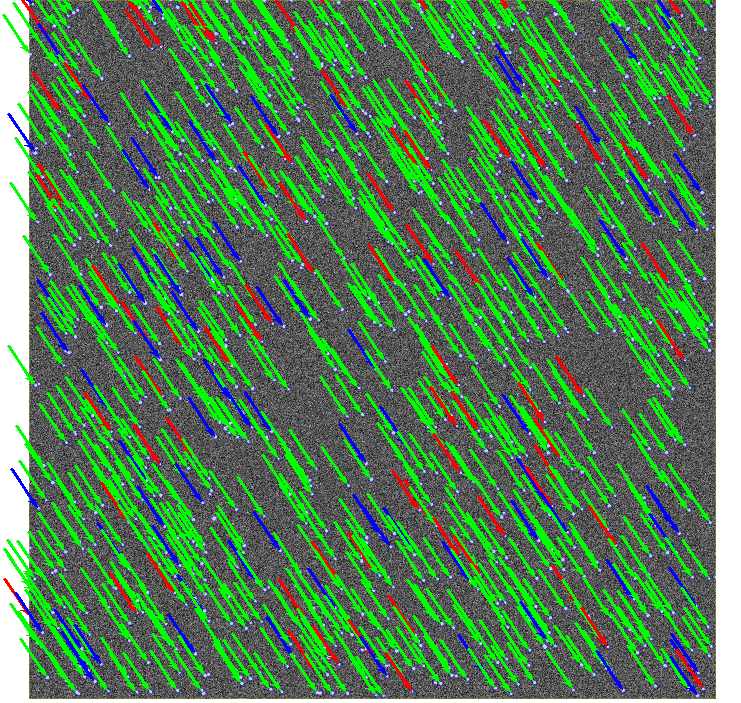
\includegraphics[width=0.5\textwidth]{\figdir/outputs8bCA_g_doPreConvolveFalse_refract_crop.png}
  \caption{{\bf Refraction}: This figure depicts the amplitude and
    orientation of the refraction vector in the visit \A, {\tt
      raft=2,2 sensor=1,1 filter=g}, seeing value {\tt 2} data.  The
    vectors point from the unrefracted locations to the realized
    locations in the image.  The SEDs of the sources are indicated
    with colors {\tt blue}, {\tt green} and {\tt red} for {\tt A0V},
    {\tt G0V}, and {\tt M2.0V} respectively.  This figure was created
    using the script {\tt python/compareDcrFromSims.py}.}
  \label{fig:refractim}
\end{figure}

\begin{figure}[h!]
  \centering
  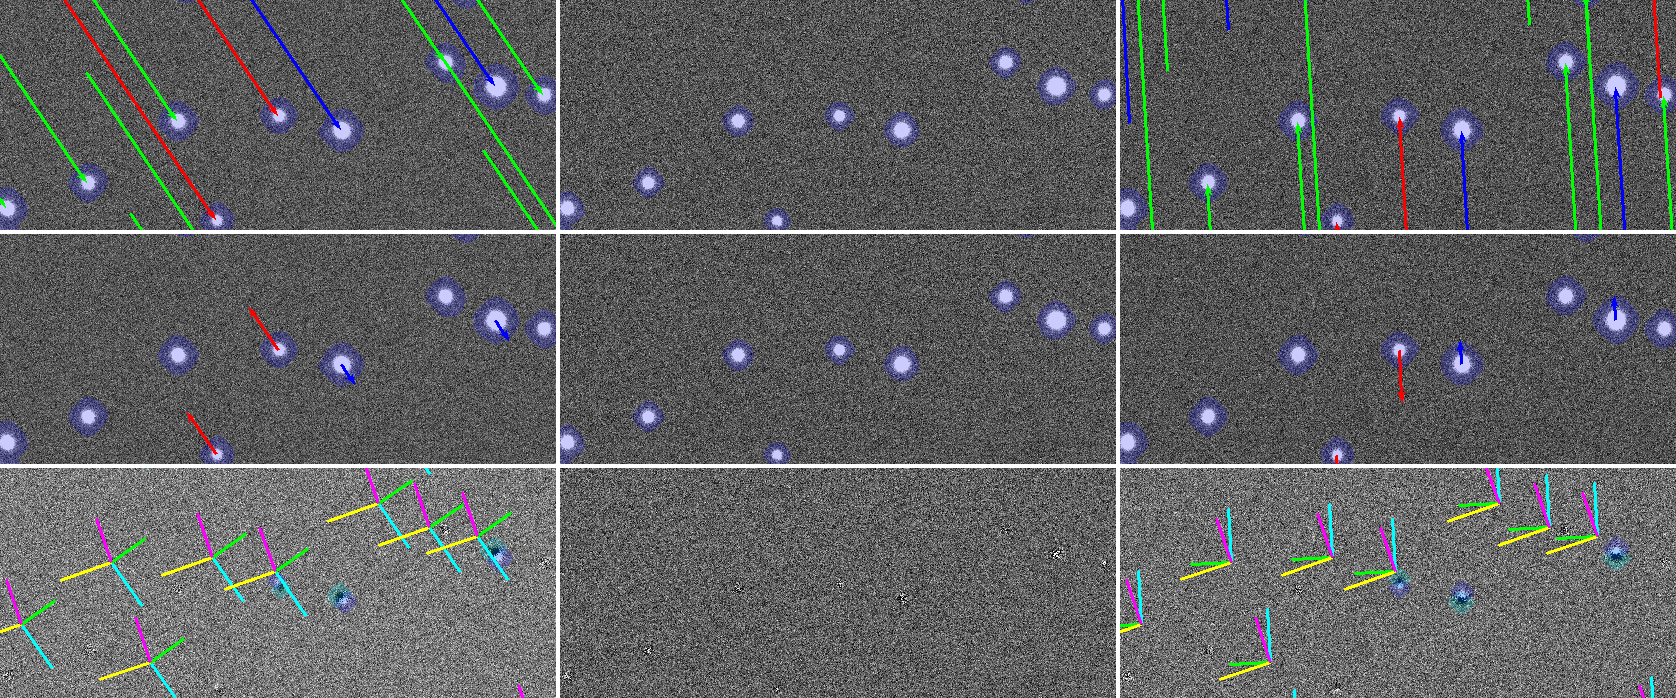
\includegraphics[width=1.0\textwidth]{\figdir/outputs8b_g_doPreConvolveFalse_dcr_crop.png}
  \caption{{\bf Differential Chromatic Refraction and Difference Image
      Quality, $g$--band}: This set of panels demonstrates the amount
    of refraction (top row), differential refraction with respect to
    the {\tt G0V} star (middle row), and the quality of the difference
    image (bottom row) for three sets of image differences.  The first
    column uses science visit \A, the middle \C, and the third \E.  In
    all cases the template used was taken at zenith, i.e. visit \C.
    The top rows effectively present the same information as
    Figure~\ref{fig:refractim}, but zoomed in on a particular cluster
    of stars.  The second row subtracts off the green vector from all
    vectors.  The residual refraction of the blue,red vectors
    represents differential chromatic refraction.  These residual
    lengths have been multiplied by a factor of 100 for readability.
    Note that the blue vectors point along the vector to zenith,
    indicating the blue stars appear higher in the sky than their
    green counterparts, compared to an unrefracted observation.  The
    red stars are not refracted as much and thus will appear lower in
    the sky.  On the bottom row, we show the realized difference image
    quality.  Note that the blue stars have positive lobes pointing
    along the direction to zenith, meaning the stars are ``higher'' in
    the sky w.r.t. the green stars when compared to the zenith
    template, while the dipoles of the red stars have the opposite
    polarity.  For completeness, the Wcs--derived orientation of the
    Ra,Decl and Az,Alt coordinate axes are shown in the difference
    image (Ra,Decl,Az,Alt are magenta,yellow,green,cyan); see
    Figure~\ref{fig:wcsdcr} for more detail.  This figure was created
    using the script {\tt python/compareDcrFromSims.py}.}
  \label{fig:dcrimg}
\end{figure}

\begin{figure}[h!]
  \centering
  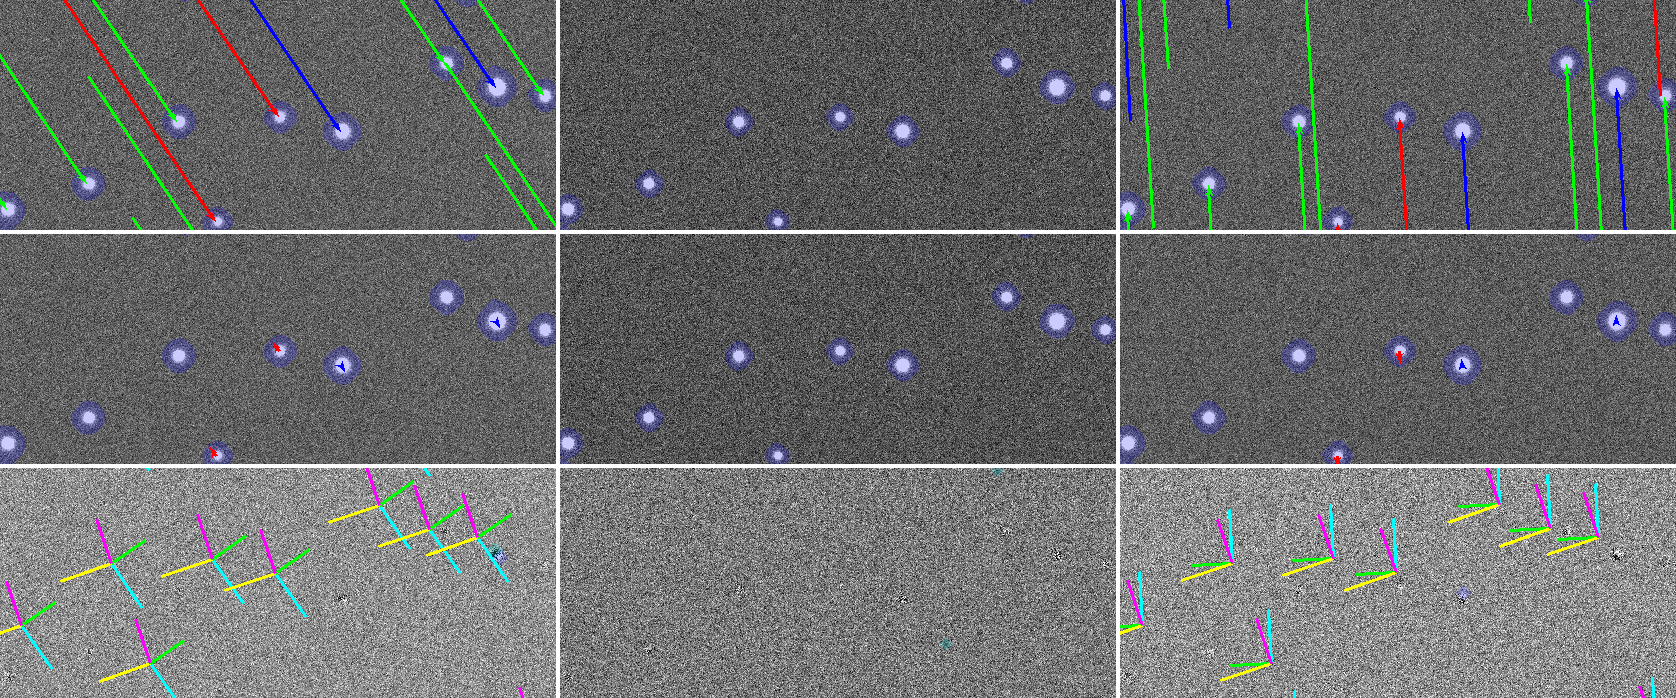
\includegraphics[width=1.0\textwidth]{\figdir/outputs8b_r_doPreConvolveFalse_dcr_crop.png}
  \caption{{\bf Differential Chromatic Refraction and Difference Image
      Quality, $r$--band}: Same as Figure~\ref{fig:dcrimg}, but for
    $r$--band data.  This figure was created using the script {\tt
      python/compareDcrFromSims.py}.}
  \label{fig:dcrimr}
\end{figure}

\begin{figure}[h!]
  \centering
  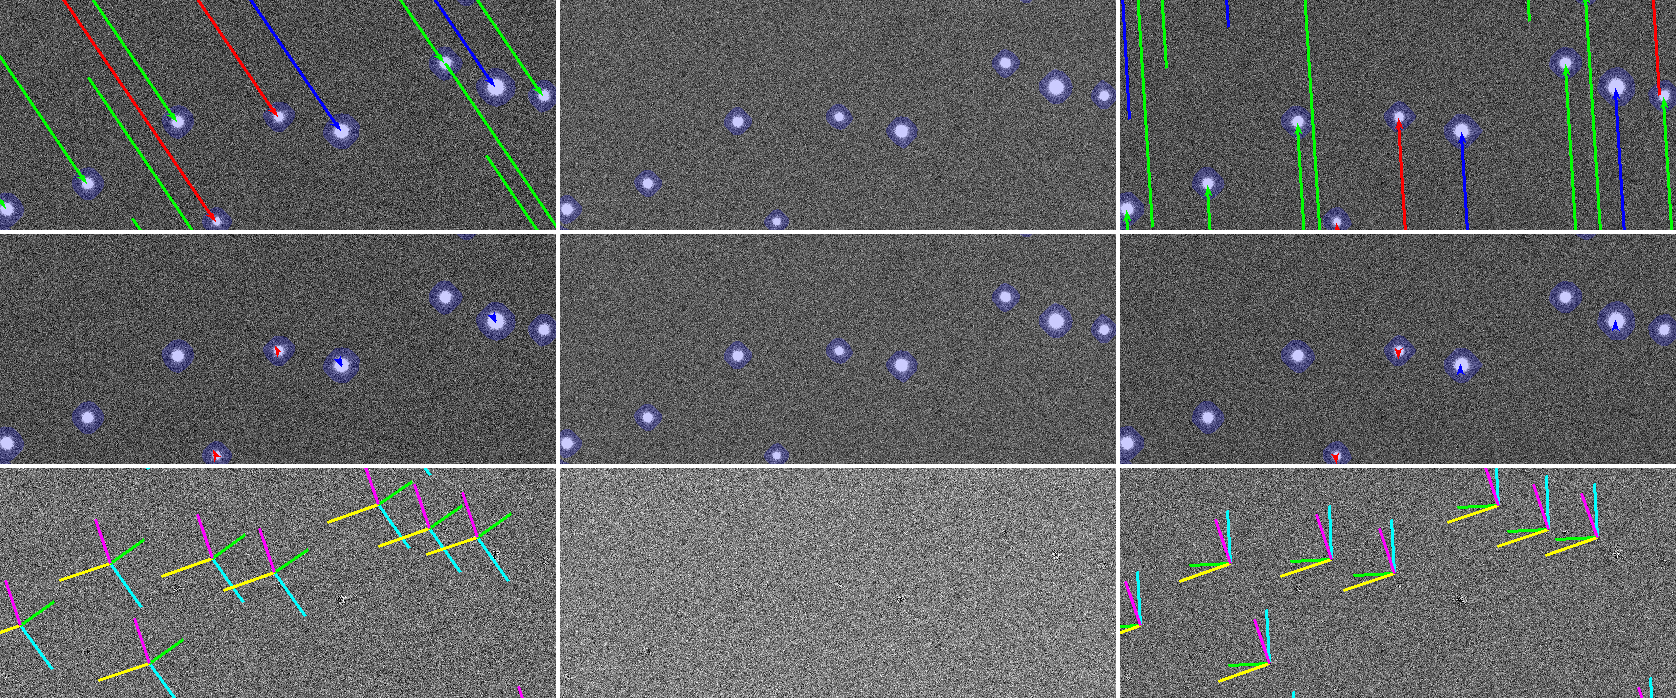
\includegraphics[width=1.0\textwidth]{\figdir/outputs8b_i_doPreConvolveFalse_dcr_crop.png}
  \caption{{\bf Differential Chromatic Refraction and Difference Image
      Quality, $i$--band}: Same as Figure~\ref{fig:dcrimg}, but for
    $i$--band data.  This figure was created using the script {\tt
      python/compareDcrFromSims.py}.}
  \label{fig:dcrimi}
\end{figure}

\begin{figure}[h!]
  \centering
  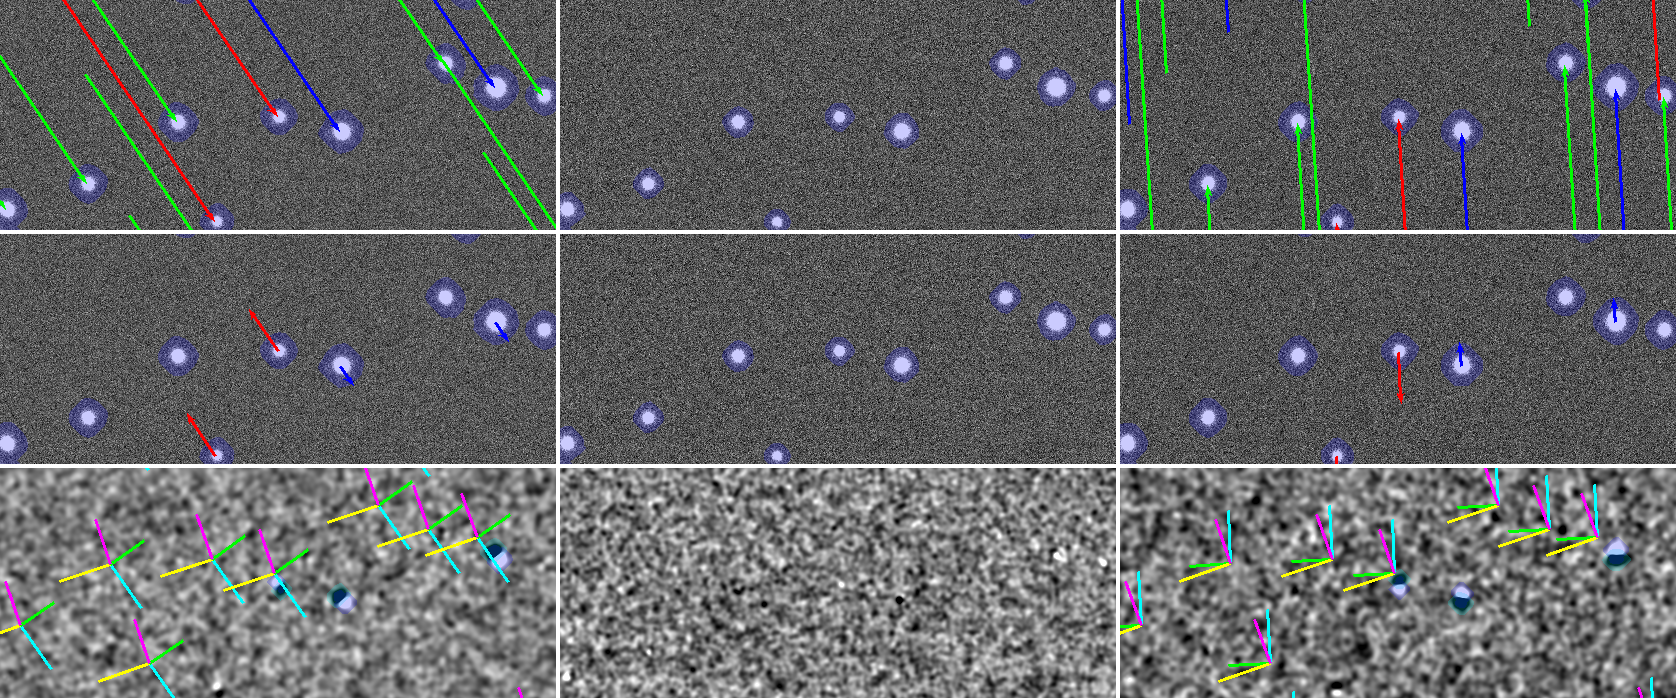
\includegraphics[width=1.0\textwidth]{\figdir/outputs8b_g_doPreConvolveTrue_dcr_crop.png}
  \caption{{\bf Differential Chromatic Refraction and Difference Image
      Quality, Prefiltering}: Same as Figure~\ref{fig:dcrimg}, but
    using prefiltering of the science image with its Psf.  This figure
    was created using the script {\tt python/compareDcrFromSims.py}.}
  \label{fig:dcrimgpre}
\end{figure}

\begin{figure}[h!]
  \centering
  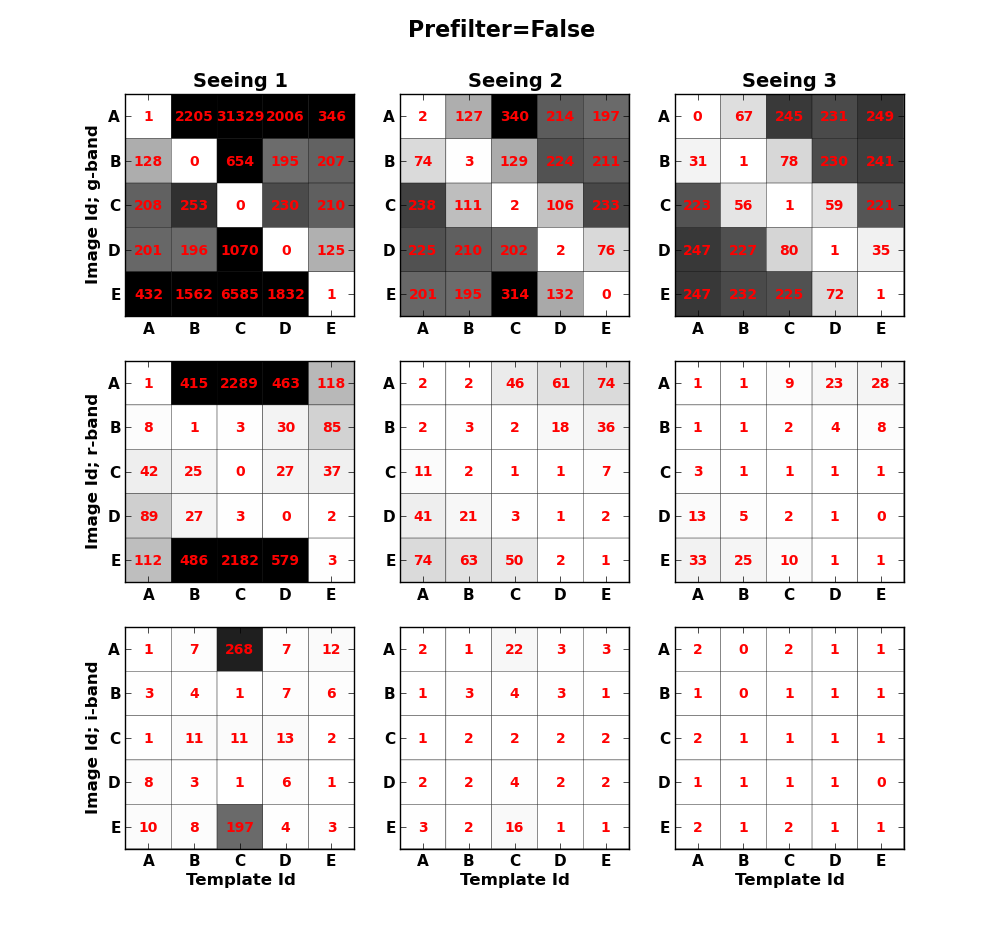
\includegraphics[width=1.0\textwidth]{\figdir/heatmapFalse.png}
  \caption{{\bf Number of False Positives, Postfiltering}: This figure
    shows the median number of false positives across the 9 {\tt
      raft=2,2} CCDs.  The first row of information shows these
    ``heat-maps'' for $g$--band data, the second for $r$--band, and
    the third for $i$--band.  The first column represents the
    good--seeing images, the second the medium--seeing images (same
    quality as template), and the third the poor-seeing images.
    Within each filter--seeing combination, the heat--map represents
    the median number of false positives as a function of the template
    airmass (visit \A\B\C\D\E) along the x--axis, and image airmass
    (visit \A\B\C\D\E) along the y--axis.  The diagonal elements
    represent the situation where the template and science image are
    taken at the same airmass and have the same orientation
    w.r.t. zenith.  The off--diagonal elements represent a mismatch
    between the template and science image in terms of airmass {\it
      and} parallactic angle.  The general trend is that the numbers
    of false positives decrease with decreasing differences in the
    airmass,angle attributes of the template and science image,
    decrease with increasing seeing, and decrease with increasing
    wavelength.  The $i$-band data in poor seeing do not appear
    sensitive to Dcr.  This figure was created using the script {\tt
      python/heatMap.py}.}
  \label{fig:heatpost}
\end{figure}

\begin{figure}[h!]
  \centering
  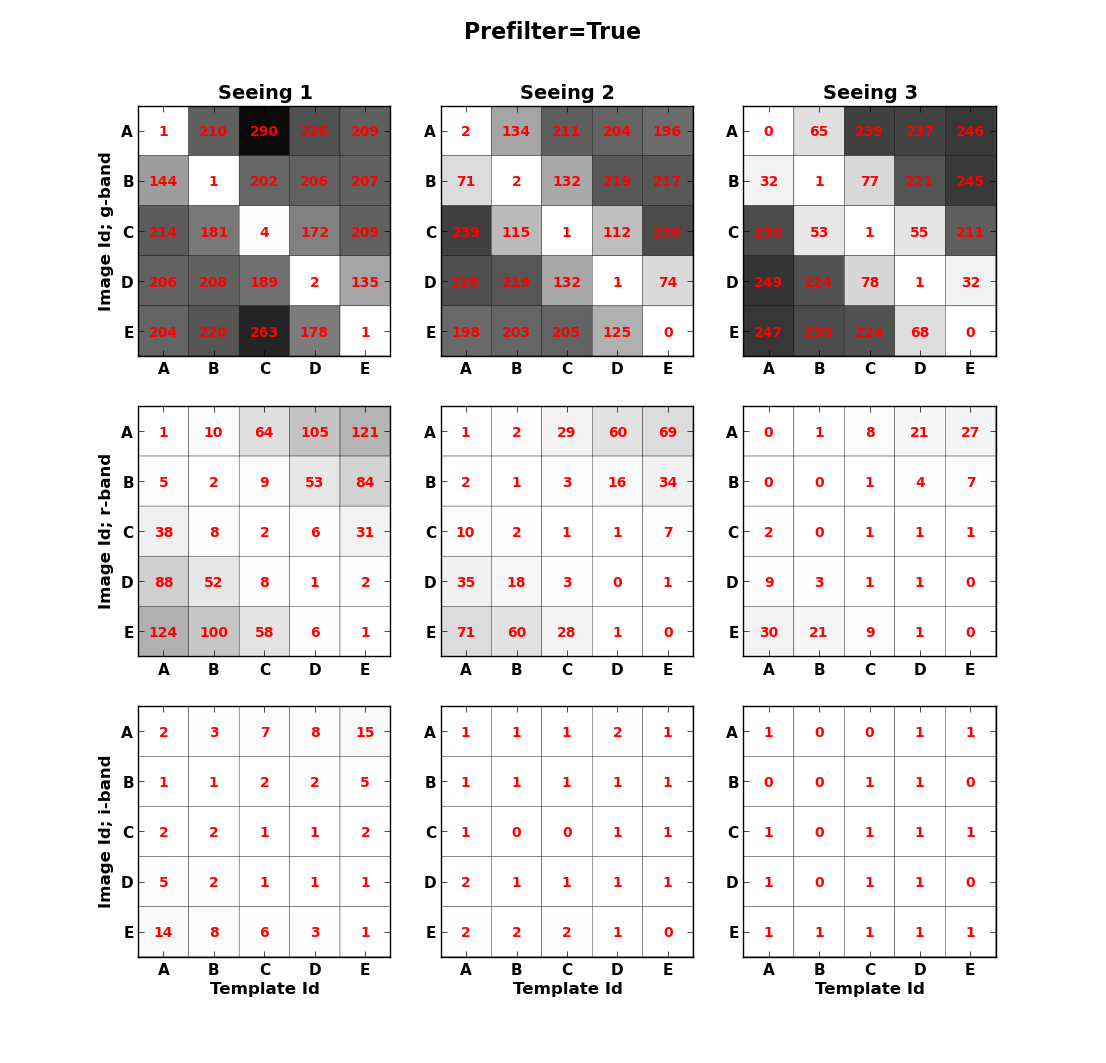
\includegraphics[width=1.0\textwidth]{\figdir/heatmapTrue.png}
  \caption{{\bf Number of False Positives, Prefiltering}: Same as
    Figure~\ref{fig:heatpost}, but using prefiltering of the science
    image with its Psf.  The numbers of false positives is overall far
    lower than in the postfiltering case (Figure~\ref{fig:heatpost}).
    This figure was created using the script {\tt python/heatMap.py}.}
  \label{fig:heatpre}
\end{figure}

\clearpage
\bibliographystyle{apj}
\bibliography{refs}

\clearpage
\begin{appendices}
\end{appendices}

\end{document}
